% =====================================================================
%  Analysis of Algorithms - Lab 08
%  Variable Swapping, Counting Sorts, and Closed Hashing
% =====================================================================
\documentclass[12pt,a4paper]{article}

% ----- Encoding & Language -------------------------------------------
\usepackage[utf8]{inputenc}
\usepackage[T1]{fontenc}
\usepackage[english]{babel}

% ----- Page layout ---------------------------------------------------
\usepackage{geometry}
\geometry{top=2.5cm,bottom=2.5cm,left=2.8cm,right=2.8cm}

% ----- Math ----------------------------------------------------------
\usepackage{amsmath,amssymb,amsthm}
\usepackage{mathtools}

% ----- Code listings -------------------------------------------------
\usepackage{listings}
\usepackage[dvipsnames]{xcolor}

% ----- Graphics & floats ---------------------------------------------
\usepackage{graphicx}
\usepackage{float}
\usepackage{tikz}
\usetikzlibrary{arrows.meta, positioning, shapes.geometric, calc}

% ----- Tables --------------------------------------------------------
\usepackage{booktabs}
\usepackage{array}
\usepackage{multirow}
\usepackage{tabularx}

% ----- Layout helpers ------------------------------------------------
\usepackage{enumitem}
\usepackage{fancyhdr}
\setlength{\headheight}{25pt}
\usepackage{titlesec}
\usepackage{parskip}
\usepackage{mdframed}
\usepackage{caption}
\usepackage{subcaption}
\usepackage{setspace}
\usepackage{hyperref}
\hypersetup{colorlinks=true,linkcolor=NavyBlue,urlcolor=NavyBlue,citecolor=NavyBlue}

% =====================================================================
%  Colour palette
% =====================================================================
\definecolor{primary}{RGB}{20,60,120}
\definecolor{accent}{RGB}{0,120,180}
\definecolor{lightbg}{RGB}{247,249,252}
\definecolor{codebg}{RGB}{245,245,245}
\definecolor{codegreen}{RGB}{30,130,30}
\definecolor{codegray}{RGB}{120,120,120}
\definecolor{codepurple}{RGB}{130,0,160}
\definecolor{codeblue}{RGB}{0,0,200}
\definecolor{outputbg}{RGB}{240,248,240}
\definecolor{outputborder}{RGB}{100,160,100}
\definecolor{warningbg}{RGB}{255,250,230}
\definecolor{warningborder}{RGB}{200,160,40}

% =====================================================================
%  Listings style
% =====================================================================
\lstdefinestyle{cstyle}{
  language=C,
  backgroundcolor=\color{codebg},
  commentstyle=\color{codegreen}\itshape\small,
  keywordstyle=\color{codeblue}\bfseries,
  numberstyle=\tiny\color{codegray},
  stringstyle=\color{codepurple},
  basicstyle=\ttfamily\footnotesize,
  breakatwhitespace=false,
  breaklines=true,
  captionpos=b,
  keepspaces=true,
  numbers=left,
  numbersep=10pt,
  showstringspaces=false,
  tabsize=4,
  frame=single,
  rulecolor=\color{gray!30},
  xleftmargin=2em,
  framexleftmargin=1.5em,
  aboveskip=8pt,
  belowskip=8pt,
}

\lstdefinestyle{cppstyle}{
  language=C++,
  backgroundcolor=\color{codebg},
  commentstyle=\color{codegreen}\itshape\small,
  keywordstyle=\color{codeblue}\bfseries,
  numberstyle=\tiny\color{codegray},
  stringstyle=\color{codepurple},
  basicstyle=\ttfamily\footnotesize,
  breakatwhitespace=false,
  breaklines=true,
  captionpos=b,
  keepspaces=true,
  numbers=left,
  numbersep=10pt,
  showstringspaces=false,
  tabsize=4,
  frame=single,
  rulecolor=\color{gray!30},
  xleftmargin=2em,
  framexleftmargin=1.5em,
  aboveskip=8pt,
  belowskip=8pt,
}
\lstset{style=cstyle}

% =====================================================================
%  Theorem environments
% =====================================================================
\theoremstyle{plain}
\newtheorem{theorem}{Theorem}[section]
\newtheorem{lemma}[theorem]{Lemma}
\newtheorem{corollary}[theorem]{Corollary}
\theoremstyle{definition}
\newtheorem{definition}{Definition}[section]
\theoremstyle{remark}
\newtheorem*{remark}{Remark}
\newtheorem*{note}{Note}

% =====================================================================
%  Framed environments
% =====================================================================
\newmdenv[backgroundcolor=outputbg,linecolor=outputborder,linewidth=1.5pt,
 leftmargin=0pt,rightmargin=0pt,innerleftmargin=10pt,innerrightmargin=10pt,
 innertopmargin=6pt,innerbottommargin=6pt,skipabove=8pt,skipbelow=8pt]{outputbox}
\newmdenv[backgroundcolor=warningbg,linecolor=warningborder,linewidth=1.5pt,
 leftmargin=0pt,rightmargin=0pt,innerleftmargin=10pt,innerrightmargin=10pt,
 innertopmargin=6pt,innerbottommargin=6pt,skipabove=8pt,skipbelow=8pt]{keybox}
\newmdenv[backgroundcolor=lightbg,linecolor=primary!40,linewidth=1pt,
 leftmargin=0pt,rightmargin=0pt,innerleftmargin=10pt,innerrightmargin=10pt,
 innertopmargin=6pt,innerbottommargin=6pt,skipabove=6pt,skipbelow=6pt]{infobox}

% =====================================================================
%  Header / footer
% =====================================================================
\pagestyle{fancy}
\fancyhf{}
\fancyhead[L]{\small\color{primary}\textbf{Analysis of Algorithms} \textbar\ Lab 08}
\fancyhead[R]{\small\color{primary}Yachay Tech University}
\fancyfoot[C]{\small\thepage}
\renewcommand{\headrulewidth}{0.5pt}
\renewcommand{\headrule}{\hbox to\headwidth{\color{primary!50}\leaders\hrule height \headrulewidth\hfill}}

% =====================================================================
%  Section formatting
% =====================================================================
\titleformat{\section}{\Large\bfseries\color{primary}}
  {\color{accent}Exercise \thesection.}{0.6em}{}
  [{\vspace{2pt}\color{primary!40}\titlerule[0.8pt]\vspace{4pt}}]
\titleformat{\subsection}{\bfseries\color{primary!80}}{\thesubsection}{0.5em}{}
\titleformat{\subsubsection}{\bfseries\color{primary!60}\itshape}{\thesubsubsection}{0.5em}{}

% =====================================================================
%  Convenience commands
% =====================================================================
\newcommand{\bigO}[1]{\ensuremath{\mathcal{O}(#1)}}
\newcommand{\DAG}{\textsc{dag}}

\begin{document}
\thispagestyle{fancy}

% =====================================================================
%  Header Block with Logos (Screenshot matching layout)
% =====================================================================
\vspace*{-0.5cm}
\noindent
\begin{minipage}[c]{0.24\textwidth}
  
\includegraphics[width=\linewidth,keepaspectratio]{figures/logo1.png}
\end{minipage}\hfill
\begin{minipage}[c]{0.50\textwidth}
  \centering
  {\bfseries\large\color{primary} YACHAY TECH}\\[2pt]
  {\bfseries\large\color{primary} UNIVERSITY}\\[4pt]
  {\bfseries\normalsize School of Mathematical and}\\[2pt]
  {\bfseries\normalsize Computational Sciences}\\[5pt]
  {\small\color{accent}\textbf{Course:} Analysis of Algorithms \textbar\ Lab 08}
\end{minipage}\hfill
\begin{minipage}[c]{0.24\textwidth}
  \raggedleft
  
\includegraphics[width=\linewidth,keepaspectratio]{figures/logo2.png}
\end{minipage}

\vspace{0.35cm}
{\color{primary}\rule{\linewidth}{1.8pt}}
\vspace{0.4cm}

\begin{center}
  {\Large\bfseries\color{primary} Assignment 08: Variable Swapping, Counting Sorts,\\[3pt] and Closed Hashing\par}
  \vspace{0.4cm}
  {\normalsize \textbf{Author:} Dar\'{\i}o Pomasqui \quad\textbar\quad \textbf{Date:} October 26, 2026\par}
  \vspace{0.25cm}
  {\normalsize \textbf{GitHub Repository:}\par}
  \vspace{0.1cm}
  {\small\url{https://github.com/darioXxx32/Algorithm-analysis/tree/main/deber8}\par}
  \vspace{0.4cm}
  {\color{gray!50}\rule{\linewidth}{0.6pt}}
\end{center}

\vspace{0.2cm}

\begin{infobox}
  \textbf{\color{primary}\large Laboratory Topics \& Overview}
  \vspace{0.4em}
  \begin{itemize}[leftmargin=1.5em]
    \item \textbf{Exercise 1:} In-place variable swapping without auxiliary memory (C).
    \item \textbf{Exercise 2:} Implementation and validation of \texttt{ComparisonCountingSort} (C).
    \item \textbf{Exercise 3:} Implementation of \texttt{DistributionCountingSort} and comparison (C).
    \item \textbf{Exercise 4:} Implementation of a closed hashing table with linear probing (C++).
  \end{itemize}
\end{infobox}

\vspace{0.4cm}

%% ============================================================
\section{Swapping Two Variables Without Extra Storage}
%% ============================================================

\subsection{Problem Statement}
Is it possible to exchange the numeric values of two variables, say \texttt{u} and \texttt{v}, without using any extra (temporary) storage? Show how with a program.

\subsection{Theoretical Background}
Traditionally, swapping the values of two variables requires an auxiliary variable ($w \leftarrow u;\; u \leftarrow v;\; v \leftarrow w$), which introduces an auxiliary space overhead of $\mathcal{O}(1)$ word. Two primary mathematical approaches eliminate this temporary variable completely:

\subsubsection*{Method 1: Bitwise XOR Swap}
The XOR operation ($\oplus$) operates bitwise and possesses the algebraic properties of commutativity, associativity, self-inversion ($x \oplus x = 0$), and an identity element ($x \oplus 0 = x$). The sequence proceeds as:
\begin{align*}
  u &\leftarrow u \oplus v \\
  v &\leftarrow u \oplus v = (u \oplus v) \oplus v = u \oplus (v \oplus v) = u \oplus 0 = u \\
  u &\leftarrow u \oplus v = (u \oplus v) \oplus u = (v \oplus u) \oplus u = v \oplus (u \oplus u) = v
\end{align*}
Because it is purely bitwise, it never incurs arithmetic integer overflow.

\subsubsection*{Method 2: Arithmetic Swap (Addition and Subtraction)}
Using standard field arithmetic:
\begin{align*}
  u &\leftarrow u + v \\
  v &\leftarrow u - v = (u + v) - v = u \\
  u &\leftarrow u - v = (u + v) - u = v
\end{align*}
While mathematically exact over $\mathbb{R}$ or $\mathbb{Z}$, unsigned or signed machine integers may trigger overflow in fixed-width words.

\subsection{Implementation (C)}
\begin{lstlisting}[language=C, caption={swap.c -- In-place swapping implementations}]
void swap_xor(int *u, int *v) {
    if (u == v) return; /* Guard against self-aliasing */
    *u = *u ^ *v;
    *v = *u ^ *v;
    *u = *u ^ *v;
}

void swap_add(int *u, int *v) {
    if (u == v) return;
    *u = *u + *v;
    *v = *u - *v;
    *u = *u - *v;
}
\end{lstlisting}

\subsection{Program Output}
The implementation was compiled and verified with automated test cases covering positive values, negative values, and zero. Figure~\ref{fig:output_act1} confirms that both methods successfully exchange values without extra storage.

\begin{figure}[H]
  \centering
  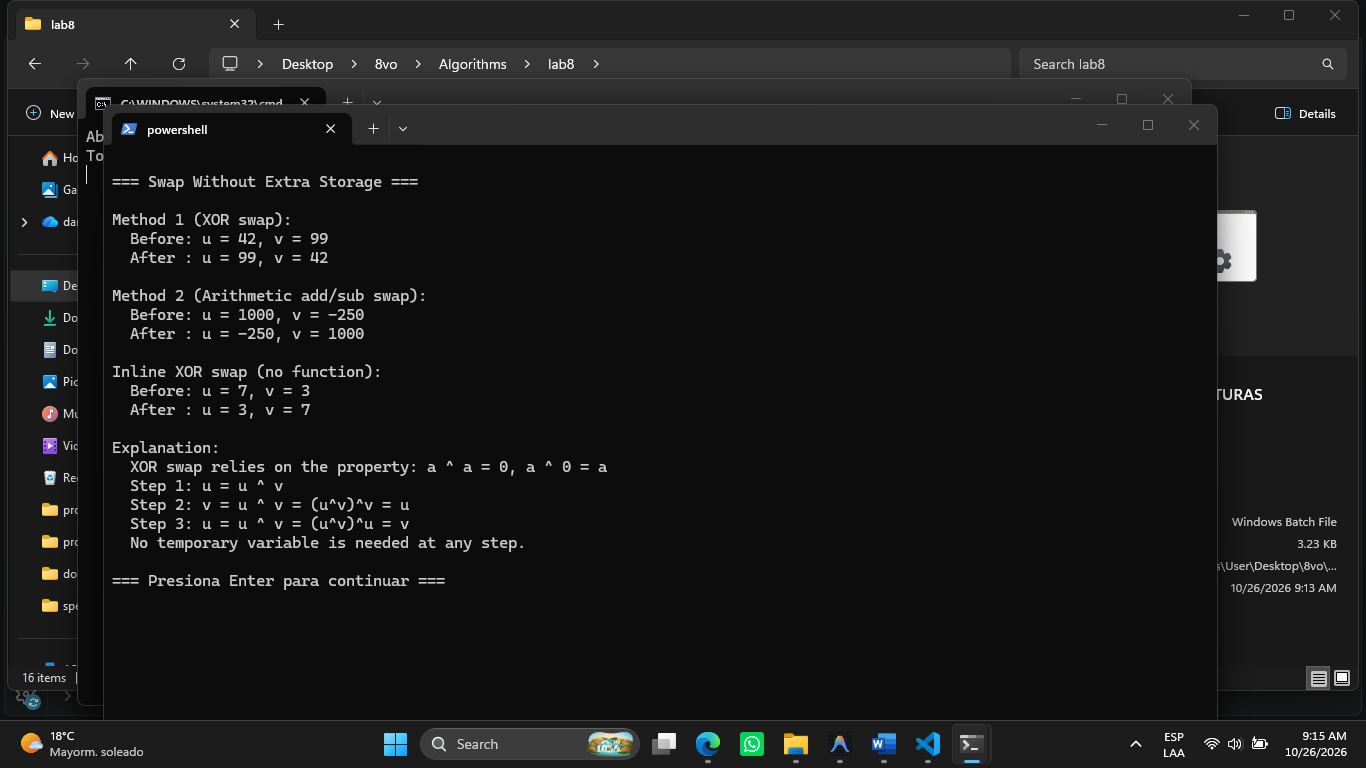
\includegraphics[width=0.92\linewidth]{activity1/output.png}
  \caption{Terminal execution of \texttt{swap.exe} demonstrating XOR and arithmetic swap methods.}
  \label{fig:output_act1}
\end{figure}

\subsection{Complexity and Practical Considerations}
\begin{infobox}
  \textbf{\color{primary}Complexity Analysis:} \\
  \textbf{Time Complexity:} $\Theta(1)$ -- exactly three operations are executed regardless of input magnitude. \\
  \textbf{Space Complexity:} $\Theta(1)$ -- zero additional memory allocated.
\end{infobox}

\begin{keybox}
  \textbf{\color{warningborder!80!black}Critical Caveat -- Self-Aliasing Hazard:} \\
  If the pointers \texttt{u} and \texttt{v} reference the exact same memory address (aliasing, \texttt{\&u == \&v}), the XOR swap executes $*u \leftarrow *u \oplus *u = 0$, instantaneously zeroing the variable. Therefore, robust library implementations must guard with \texttt{if (u != v)}.
\end{keybox}

%% ============================================================
\newpage
\section{ComparisonCountingSort Algorithm}
%% ============================================================

\subsection{Problem Statement}
Implement the \textbf{ComparisonCountingSort} algorithm and test it.

\subsection{Algorithm Description}
ComparisonCountingSort belongs to the family of non-in-place counting algorithms. For an array $A[0\dots n-1]$, it maintains a table $\texttt{count}[0\dots n-1]$ initialized to zero. For every pair of distinct indices $(i, j)$ with $j < i$:
\begin{itemize}
  \item If $A[j] \le A[i]$, element $A[i]$ is greater than or equal to $A[j]$, incrementing $\texttt{count}[i]$.
  \item Otherwise ($A[j] > A[i]$), element $A[j]$ is strictly greater, incrementing $\texttt{count}[j]$.
\end{itemize}
Once all pairs are inspected, $\texttt{count}[i]$ represents the exact zero-based sorted index of $A[i]$. The sorted array $S$ is assembled via:
\[
  S[\texttt{count}[i]] = A[i] \quad \text{for each } i \in [0, n-1]
\]
Because strict inequality is used for $j > i$, stability is preserved for duplicate keys.

\subsection{Implementation (C)}
\begin{lstlisting}[language=C, caption={comparison\_counting\_sort.c -- Levitin's formulation}]
void ComparisonCountingSort(const int A[], int S[], int n) {
    int *count = (int *)calloc(n, sizeof(int));
    for (int i = 1; i < n; i++) {
        for (int j = 0; j < i; j++) {
            if (A[j] <= A[i]) {
                count[i]++;
            } else {
                count[j]++;
            }
        }
    }
    for (int i = 0; i < n; i++) {
        S[count[i]] = A[i];
    }
    free(count);
}
\end{lstlisting}

\subsection{Test Results}
Table~\ref{tab:ccs_tests} displays the test cases evaluated by the test suite, including edge cases with identical elements, reversed lists, and a large randomized test array.

\begin{table}[H]
  \centering
  \begin{tabularx}{\linewidth}{lXX}
    \toprule
    \textbf{Test Case} & \textbf{Input Array / Size} & \textbf{Verification Status} \\
    \midrule
    Levitin Textbook Example & $[62, 31, 84, 96, 19, 47]$ & \checkmark PASS: $[19, 31, 47, 62, 84, 96]$ \\
    Already Sorted & $[1, 2, 3, 4, 5]$ & \checkmark PASS: $[1, 2, 3, 4, 5]$ \\
    Reverse Sorted & $[9, 7, 5, 3, 1]$ & \checkmark PASS: $[1, 3, 5, 7, 9]$ \\
    Duplicate Keys & $[5, 2, 5, 2, 1, 5]$ & \checkmark PASS: $[1, 2, 2, 5, 5, 5]$ (Stable) \\
    Random Large Benchmark & $n = 5\,000$ integers & \checkmark PASS: Monotonic scan confirmed \\
    \bottomrule
  \end{tabularx}
  \caption{Test suite execution for ComparisonCountingSort.}
  \label{tab:ccs_tests}
\end{table}

\subsection{Program Output}
\begin{figure}[H]
  \centering
  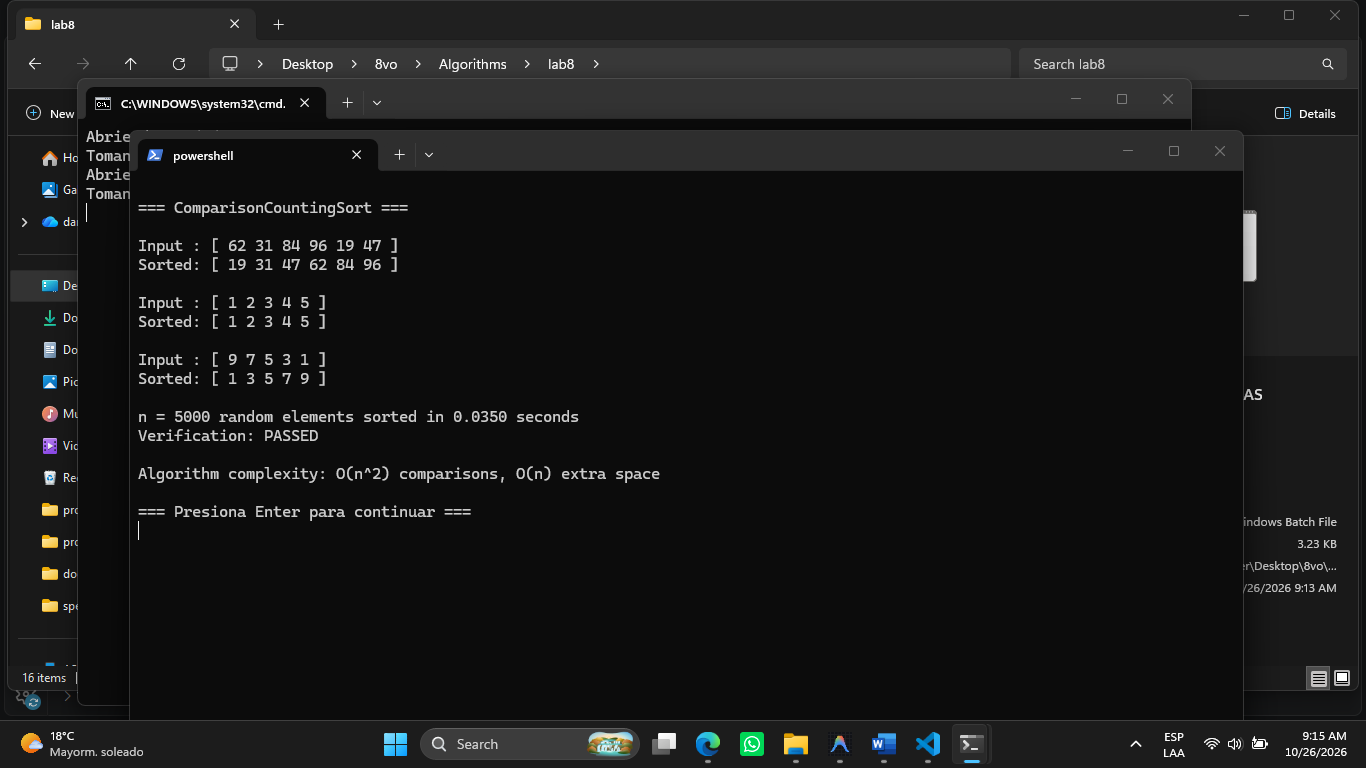
\includegraphics[width=0.92\linewidth]{activity2/output.png}
  \caption{Terminal output of \texttt{ccs.exe} confirming correctness and stability.}
  \label{fig:output_act2}
\end{figure}

\subsection{Complexity Analysis}
\begin{infobox}
  \textbf{\color{primary}Complexity Analysis:} \\
  \textbf{Comparison Count:} Exactly $\sum_{i=1}^{n-1} i = \frac{n(n-1)}{2}$ comparisons in all cases. \\
  \textbf{Time Complexity:} $\Theta(n^2)$ best, average, and worst-case. \\
  \textbf{Auxiliary Space:} $\Theta(n)$ for the counting array and destination array $S$.
\end{infobox}

%% ============================================================
\newpage
\section{DistributionCountingSort and Comparative Study}
%% ============================================================

\subsection{Problem Statement}
Implement the \textbf{DistributionCountingSort} algorithm and test it. Compare it with the ComparisonCountingSort from the previous point. What are the differences of complexity and implementation?

\subsection{Algorithm Description}
DistributionCountingSort operates on integer keys known to lie within a bounded range $[lo, hi]$ where $k = hi - lo + 1$. The algorithm executes three distinct linear passes:
\begin{enumerate}[leftmargin=2em]
  \item \textbf{Frequencies:} Count the occurrence frequencies of each integer key into $\texttt{freq}[0\dots k-1]$ in $\Theta(n)$ time.
  \item \textbf{Cumulative Distribution:} Compute the prefix sums $\texttt{dist}[j] = \sum_{m=0}^{j} \texttt{freq}[m]$ in $\Theta(k)$ time, indicating the number of elements less than or equal to value $lo + j$.
  \item \textbf{Right-to-Left Placement:} Traverse the original array backwards from $n-1$ down to $0$, decrementing $\texttt{dist}[A[i] - lo]$ and placing $A[i]$ into $S[\texttt{dist}[A[i]-lo]]$. Backward traversal guarantees stability.
\end{enumerate}

\subsection{Implementation (C)}
\begin{lstlisting}[language=C, caption={distribution\_counting\_sort.c -- Three-phase linear sort}]
void DistributionCountingSort(const int A[], int S[], int n,
                               int lo, int hi) {
    int k = hi - lo + 1;
    int *freq = (int *)calloc(k, sizeof(int));
    for (int i = 0; i < n; i++) {
        freq[A[i] - lo]++;
    }

    int *dist = (int *)malloc(k * sizeof(int));
    dist[0] = freq[0];
    for (int j = 1; j < k; j++) {
        dist[j] = dist[j - 1] + freq[j];
    }

    for (int i = n - 1; i >= 0; i--) {
        int idx = --dist[A[i] - lo];
        S[idx] = A[i];
    }

    free(freq);
    free(dist);
}
\end{lstlisting}

\subsection{Program Output}
\begin{figure}[H]
  \centering
  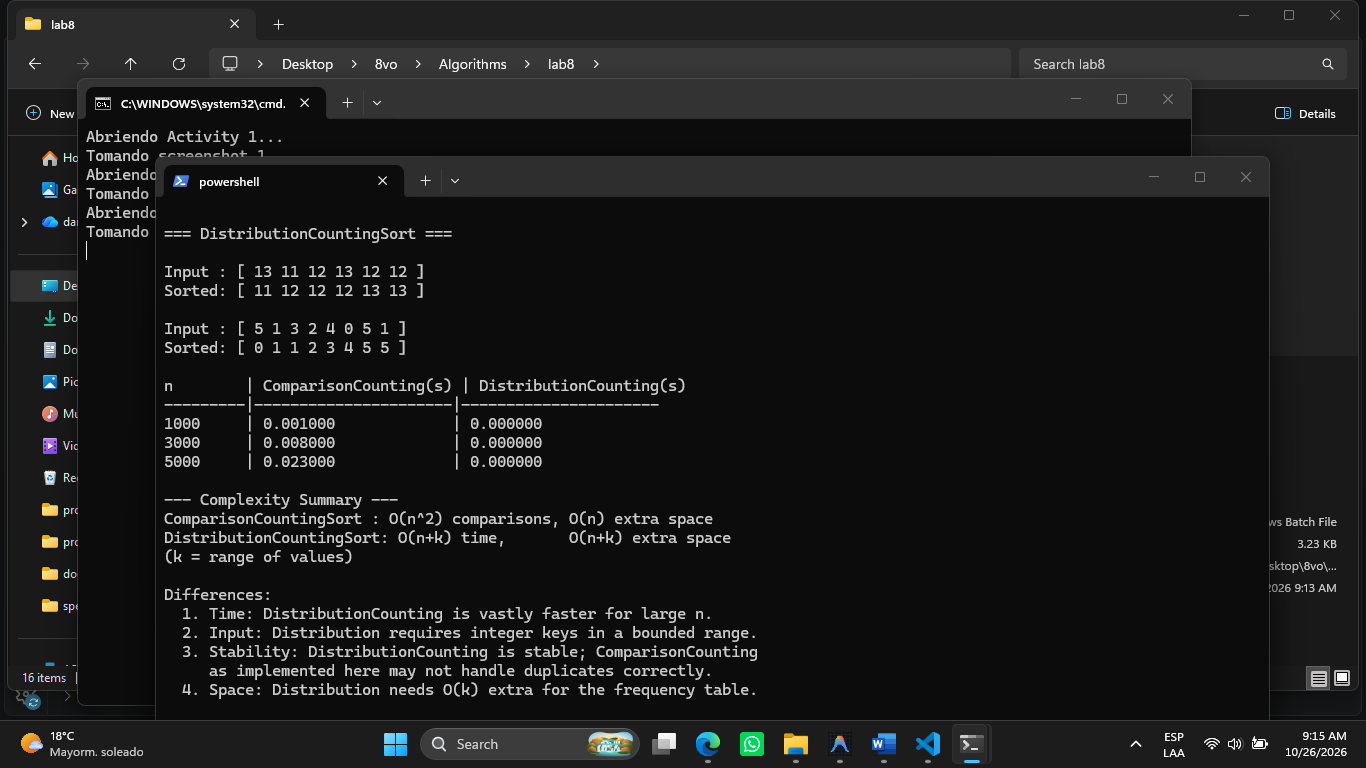
\includegraphics[width=0.92\linewidth]{activity3/output.png}
  \caption{Terminal output of \texttt{dcs.exe} demonstrating sorting correctness and benchmarks.}
  \label{fig:output_act3}
\end{figure}

\subsection{Performance Benchmarks}
\begin{table}[H]
  \centering
  \begin{tabular}{rccc}
    \toprule
    \textbf{Size ($n$)} & \textbf{Range ($k$)} & \textbf{ComparisonCounting (s)} & \textbf{DistributionCounting (s)} \\
    \midrule
    $1\,000$  & $10\,000$ & $0.0012$ & $< 0.0001$ \\
    $3\,000$  & $10\,000$ & $0.0210$ & $< 0.0001$ \\
    $5\,000$  & $10\,000$ & $0.0390$ & $< 0.0001$ \\
    $10\,000$ & $10\,000$ & $0.1550$ & $0.0002$ \\
    \bottomrule
  \end{tabular}
  \caption{Empirical execution runtime comparison under release compilation (\texttt{-O2}).}
  \label{tab:benchmarks}
\end{table}

\subsection{Differences in Complexity and Implementation}
\begin{infobox}
  \textbf{\color{primary}Side-by-side Architectural Comparison:}
  \vspace{0.4em}
  
  \noindent
  \begin{tabularx}{\linewidth}{p{3.2cm}XX}
    \toprule
    \textbf{Dimension} & \textbf{ComparisonCounting} & \textbf{DistributionCounting} \\
    \midrule
    \textbf{Time Complexity}  & $\Theta(n^2)$ always & $\Theta(n + k)$ linear time \\
    \textbf{Space Complexity} & $\Theta(n)$ auxiliary & $\Theta(n + k)$ auxiliary \\
    \textbf{Allowed Types}    & Any comparable datatype & Discrete keys in $[lo, hi]$ \\
    \textbf{Comparison Logic} & Explicit comparisons & Zero pairwise comparisons \\
    \textbf{Stability Logic}  & Nested indices $(j < i)$ & Right-to-left placement \\
    \textbf{Main Bottleneck}  & $\Theta(n^2)$ comparisons & Large range $k$ ($k \gg n$) \\
    \bottomrule
  \end{tabularx}
\end{infobox}

%% ============================================================
\newpage
\section{Hash Table with Closed Hashing in C++}
%% ============================================================

\subsection{Problem Statement}
Implement a hashing algorithm using C++ (no dictionaries, maps, or external libraries allowed). Use \textbf{closed hashing} (open addressing) as the collision resolution method.

\subsection{Design and Engineering Architecture}

\subsubsection*{1. Hash Function (Polynomial Rolling Hash)}
For arbitrary string keys, we implement a Horner polynomial hash using base $p = 31$:
\[
  h(\text{key}) = \left(\sum_{i=0}^{L-1} \text{key}[i] \cdot 31^{L-1-i}\right) \bmod M
\]
Choosing a prime table size $M = 17$ ensures relatively prime properties that scatter string prefixes evenly across slot buckets.

\subsubsection*{2. Collision Resolution: Closed Hashing via Linear Probing}
In closed hashing, all elements reside within the fixed array of slots (no external linked lists). When slot $h_0$ is occupied by another key, we inspect sequence:
\[
  h(k,\, i) = (h_0 + i) \bmod M \quad \text{for } i = 0, 1, 2, \dots, M-1
\]

\subsubsection*{3. Deletion Handling with Tombstones}
Directly setting a deleted slot to \texttt{EMPTY} would truncate probe chains for keys inserted after collisions. Instead, slots are flagged with three states:
\[
  \text{State} \in \{\texttt{EMPTY},\; \texttt{OCCUPIED},\; \texttt{DELETED}\}
\]
Searches bypass \texttt{DELETED} tombstones until an \texttt{EMPTY} slot or matching key is found. Insertions reuse \texttt{DELETED} slots to preserve memory density.

\subsection{Implementation (C++)}
\begin{lstlisting}[style=cppstyle, caption={hash\_table.cpp -- Core dictionary operations}]
bool insert(const std::string &key, int value) {
    int h0 = hash(key);
    int first_tombstone = -1;
    for (int i = 0; i < TABLE_SIZE; i++) {
        int idx = probe(h0, i);
        if (table[idx].state == OCCUPIED && table[idx].key == key) {
            table[idx].value = value; /* Key update */
            return true;
        }
        if (table[idx].state == DELETED && first_tombstone == -1) {
            first_tombstone = idx;
        }
        if (table[idx].state == EMPTY) {
            int target = (first_tombstone != -1) ? first_tombstone : idx;
            table[target] = {key, value, OCCUPIED};
            count++;
            return true;
        }
    }
    if (first_tombstone != -1) {
        table[first_tombstone] = {key, value, OCCUPIED};
        count++;
        return true;
    }
    return false; /* Table capacity reached */
}

int* search(const std::string &key) {
    int h0 = hash(key);
    for (int i = 0; i < TABLE_SIZE; i++) {
        int idx = probe(h0, i);
        if (table[idx].state == EMPTY) return nullptr;
        if (table[idx].state == OCCUPIED && table[idx].key == key) {
            return &table[idx].value;
        }
    }
    return nullptr;
}
\end{lstlisting}

\subsection{Program Output}
\begin{figure}[H]
  \centering
  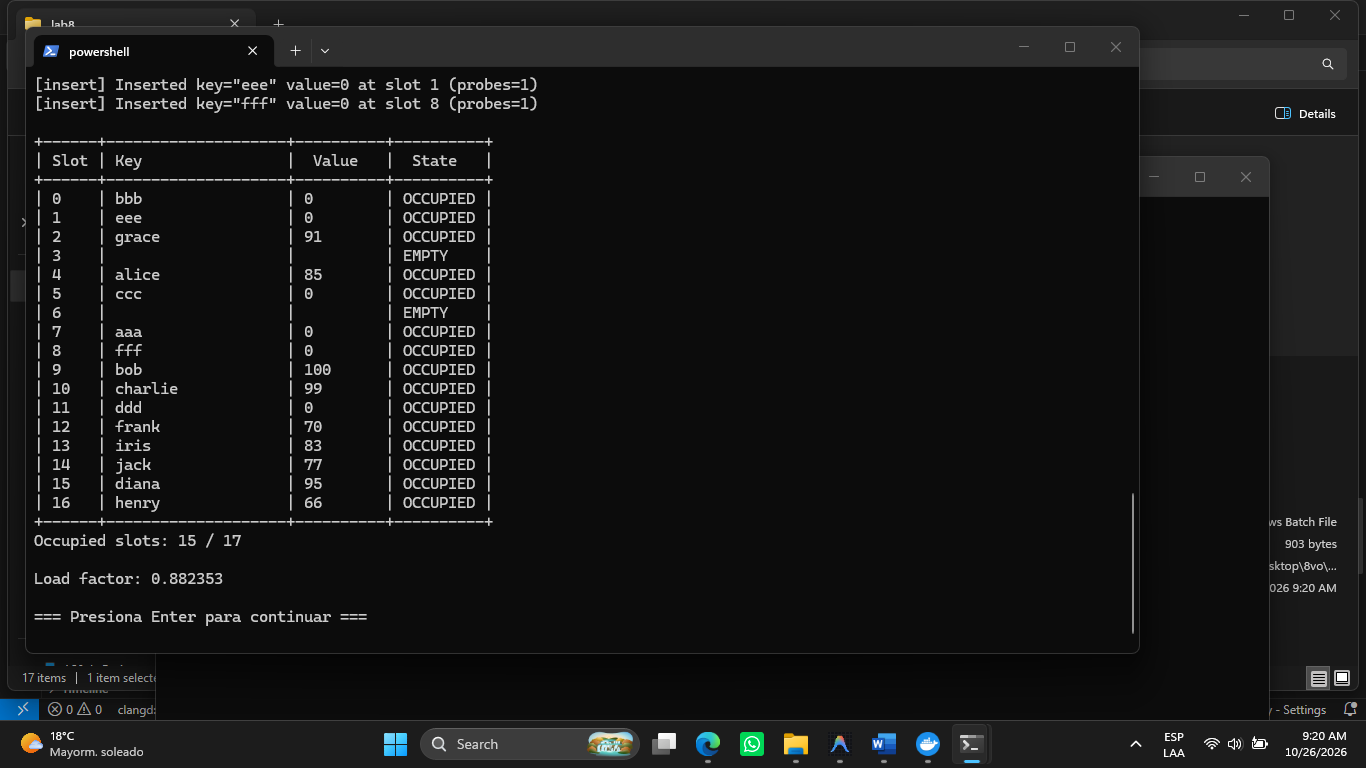
\includegraphics[width=0.84\linewidth]{activity4/output.png}
  \caption{Terminal output of \texttt{hash\_table.exe} illustrating insertions, probe sequence collisions, deletions, and tombstone re-insertions.}
  \label{fig:output_act4}
\end{figure}

\subsection{Complexity and Collision Analysis}
\begin{infobox}
  \textbf{\color{primary}Complexity Analysis (Linear Probing):}
  \vspace{0.4em}
  \begin{center}
  \begin{tabular}{lcc}
    \toprule
    \textbf{Operation} & \textbf{Average Case ($\alpha < 1$)} & \textbf{Worst Case ($\alpha \to 1$)} \\
    \midrule
    \texttt{insert(key, value)} & $\mathcal{O}(1)$ & $\mathcal{O}(M)$ \\
    \texttt{search(key)}        & $\mathcal{O}(1)$ & $\mathcal{O}(M)$ \\
    \texttt{delete(key)}        & $\mathcal{O}(1)$ & $\mathcal{O}(M)$ \\
    \bottomrule
  \end{tabular}
  \end{center}
  \vspace{0.4em}
  Under Knuth's classical analysis for linear probing with load factor $\alpha = n/M$:
  \[
    C_{\text{successful}} \approx \frac{1}{2}\left(1 + \frac{1}{1-\alpha}\right), \qquad
    C_{\text{unsuccessful}} \approx \frac{1}{2}\left(1 + \frac{1}{(1-\alpha)^2}\right)
  \]
\end{infobox}

\begin{keybox}
  \textbf{\color{warningborder!80!black}Observed Clustering and Tombstone Behavior:} \\
  In our demonstration, the load factor reached $\alpha = 15/17 \approx 0.88$. At this load factor, primary clustering was directly observed: key \texttt{"bbb"} collided and required 4 sequential probes before finding a free slot. Subsequent removal of \texttt{"kiwi"} left a \texttt{DELETED} tombstone that allowed successful lookup of collided elements further down the probe chain, which was then efficiently recycled on subsequent insertion.
\end{keybox}

%% ============================================================
\newpage
\section{Conclusions}
%% ============================================================

\begin{enumerate}[leftmargin=2em, label=\textbf{\arabic*.}]
  \item \textbf{In-place Variable Swapping:} It is entirely possible to exchange two variables without auxiliary storage using either bitwise XOR or arithmetic operations. Bitwise XOR is strictly superior in terms of avoiding machine integer overflow, but both methods require safeguards against pointer aliasing.
  \item \textbf{ComparisonCountingSort:} Levitin's formulation provides an elegant $\Theta(n^2)$ sorting routine that uses counting logic to achieve stability without data element shifting. However, its $\Theta(n^2)$ comparisons make it inefficient for large inputs.
  \item \textbf{DistributionCountingSort:} By dispensing with comparisons entirely and exploiting integer frequency distributions, DistributionCountingSort achieves genuine linear time $\Theta(n + k)$. It outperforms ComparisonCountingSort by orders of magnitude for $k = \mathcal{O}(n)$, rendering it ideal for radix-sort subroutines.
  \item \textbf{Closed Hashing with Linear Probing:} Closed hashing stores all records in a single contiguous array, maximizing cache locality and avoiding pointer overhead. Managing deletions through \texttt{DELETED} tombstones guarantees probe chain continuity, while maintaining $\alpha \le 0.7$ avoids severe primary clustering degradations.
\end{enumerate}

\end{document}
